\documentclass[12pt]{kiarticle} % You can learn about my document class "kiarticle" and install it to your device by following the link: https://github.com/Kiarendil/toolkitex
\graphicspath{{pictures/}}
\DeclareGraphicsExtensions{.pdf,.png,.jpg,.eps}
%%%
\pagestyle{fancy}
\fancyhf{}
%\renewcommand{\headrulewidth}{ 0.1mm }
\renewcommand{\footrulewidth}{ .0em }
\fancyfoot[C]{\texttt{\textemdash~\thepage~\textemdash}}
\fancyhead[L]{Лабораторная работа № 6.11.2 \hfil}
\fancyhead[R]{\hfil Иванов Кирилл, 625 группа }
\usepackage{multirow} % Слияние строк в таблице
\newcommand
{\un}[1]
{\ensuremath{\text{#1}}}
\newcommand{\eds}{\ensuremath{ \mathscr{E}}}
\newcommand{\ga}{\ensuremath{\gamma}}
\newcommand{\an}{\ensuremath{\mathring{A}}}
\usepackage{tikz}
%%% Работа с таблицами
\usepackage{array,tabularx,tabulary,booktabs} % Дополнительная работа с таблицами
\usepackage{longtable}  % Длинные таблицы
\usepackage{multirow} % Слияние строк в таблице

\begin{document}
	
	\begin{titlepage}
		\begin{center}
			\large 	Московский физико-технический институт \\
				(национальный исследовательский университет) \\
			Факультет общей и прикладной физики \\
			\vspace{0.2cm}
			
			\vspace{4.5cm}
			Лабораторная работа №6.11.2 \\ \vspace{0.2cm}
			\large (Общая физика: квантовая физика) \\ \vspace{0.2cm}
			\LARGE \textbf{Исследование фотопроводимости полупроводников}
		\end{center}
		\vspace{2.3cm} \large
		
		\begin{center}
			Работу выполнил: \\
			Иванов Кирилл,
			625 группа
			\vspace{10mm}		
			
		\end{center}
		
		\begin{center} \vspace{60mm}
			г. Долгопрудный \\
			2018 год
		\end{center}
	\end{titlepage}


	\paragraph*{Цель работы:} исследовать собственную фотопроводимость. По полученной спектральной зависимости фототока определить ширину запрещенной зоны.
	
	
	
	\section{Теоретическое введение}
	
	Электропроводность полупроводника увеличивается под действием света. Это явление называется \textbf{фотопроводимостью} или {внутренним фотоэффектом}. 
	
	В отсутствии света в полупроводнике присутствует некоторое количество носителей тока: электроны переходя из валентной зоны в зону проводимости (в случае наличия примесей возможны также переходы с донорных на акцепторные уровни) в результате теплового движения. Количество таких носителей определяется температурой кристалла, они называются равновесными и составляют темновой ток. 
	
	Фотопроводимость проявляется в случае, если энергия квантов превышает некоторое пороговое значение. Для собственной фотопроводимости это значение равно ширине запрещенной зоны, а в случае примесной --- энергии ионизации соответствующего уровня. Минимальная частота света, при которой возможно появление неравновесных электронов (то есть, электронов фотопроводимости), называется красной границей фотоэффекта. При этом можно считать, что включение света не влияет на концентрацию равновесных электронов. 
	

	\section{Экспериментальная установка}
	
	В работе исследуются два образца: CdS и CdSe. Схема установки приведена на рисунке \ref{pic:scheme}. Свет от источника И с помощью линзы Л фокусируется на щель монохроматора УМ-2, находящуюся в фокусе линзы Л$_1$. Пучое света разлагается призмой П, и выходная щель, находящаяся в фокусе линзы Л$_2$, вырезает отпределенную область спектра. После прохождения монохроматора свет падает на ячейку Я с образцом. Вольтметр В7-34 нужен для измерения тока через образец. 
	
	\begin{figure}[h]
		\centering	
		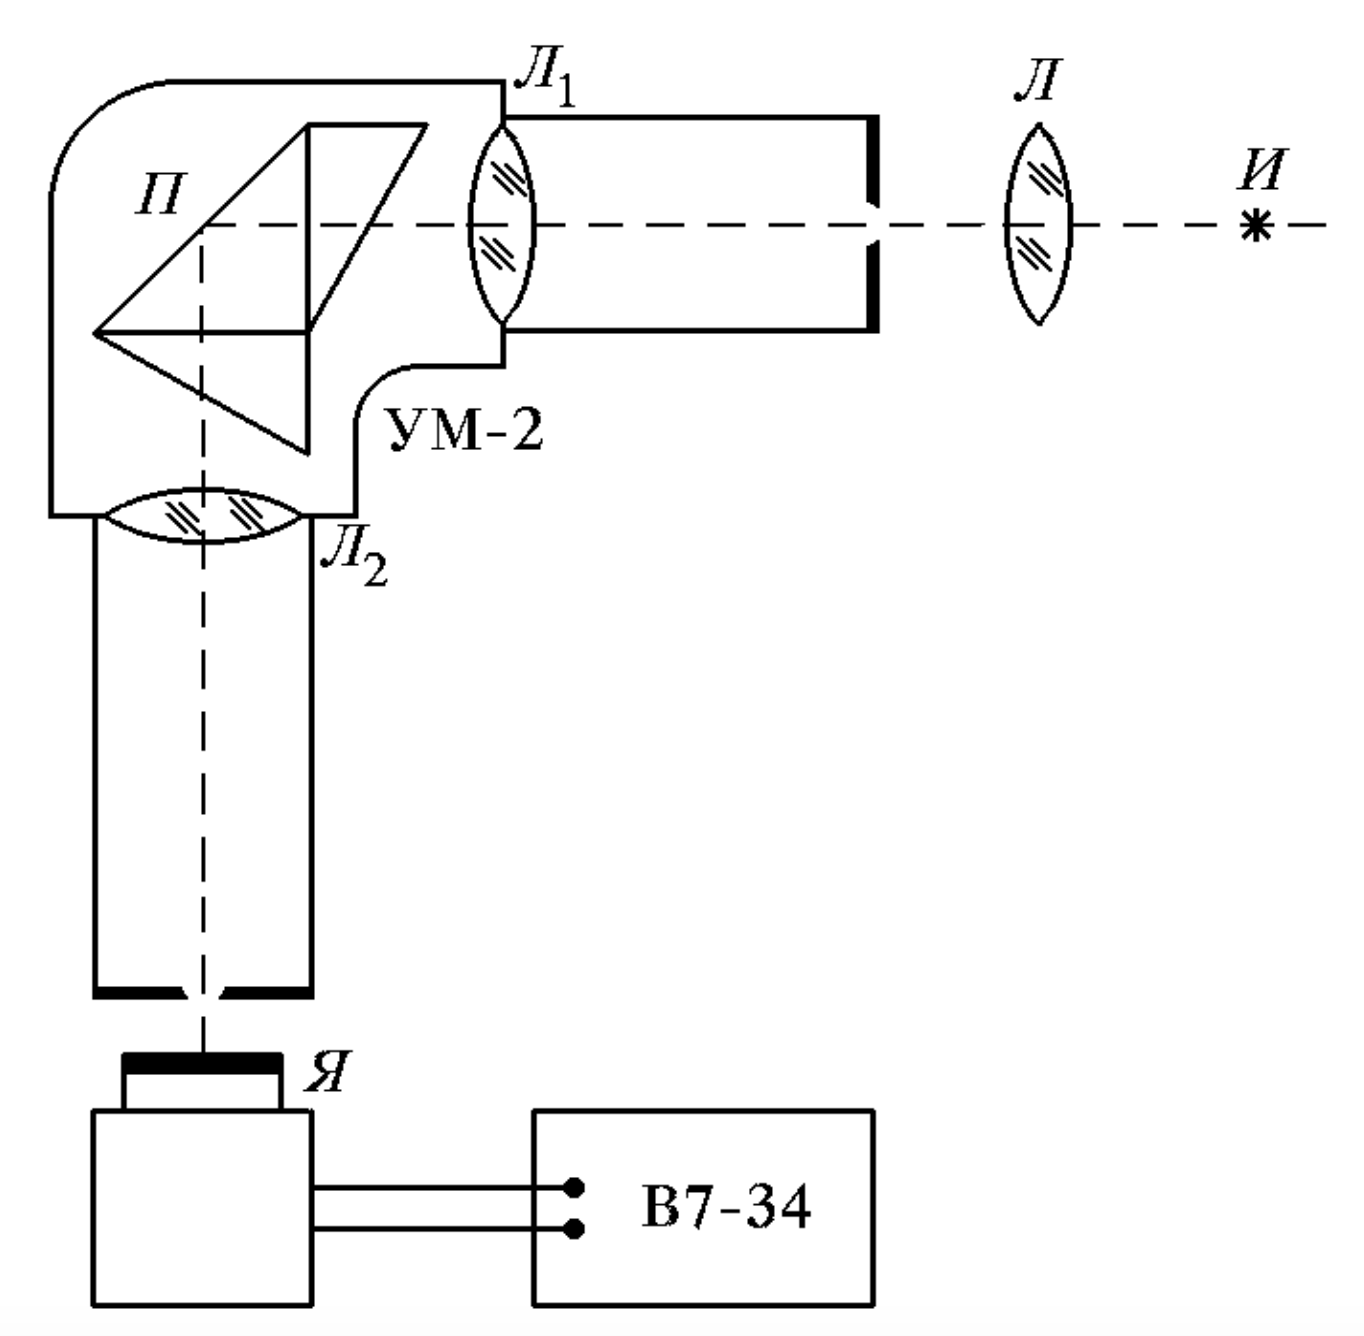
\includegraphics[width=0.4\textwidth]{lab.png}
		\caption{Схема установки для исследования спектральной зависимости фототока}
		\label{pic:scheme}
	\end{figure} 
	
	Спектральное распределение потока фотонов на выходе монохроматора и его градиуровочная кривая приведены на рисунке \ref{pic:calib}.
	
	\begin{figure}[h]
		\centering	
		\includegraphics[width=\textwidth]{scan}
		\caption{Спектральное распределение потока фотонов на выходе монохроматора и его градуировочная кривая}
		\label{pic:calib}
	\end{figure}
	
	
	\section{Выполнение работы}
	
	Прежде чем приступать к основным измерениям, уточним известную градуировочную кривую монохроматора: для ярких линий спектра неоновой лампы найдем соответствующие положения барабана. Измерения зафиксированы в таблице \ref{tab:calib}. Из анализа этих измерений, градуировочную кривую нужно <<сдвинуть влево>> примерно на 520 делений.
	
	\begin{table}[h]
		\centering
		\caption{Зависимость угла поворота $\varphi$ барабана монохроматора от наблюдаемой линии $\lambda$}
		\begin{tabular}{|c|c|c|c|}
			\hline 
			Цвет & $ \lambda_n, \an $  & $ \phi $ & $ \lambda, \mathring{A} $ \\ 
			\hline 
			Зеленый& 5400 &  1890 & 4945 \\ 
			\hline 
			Желтый & 5842 & 2152 & 5291 \\ 
			\hline 
			Красный & 6217 & 2392 & 5667  \\ 
			\hline 
		\end{tabular} 
	\end{table}
	
	Перейдем теперь к основным измерениям, и заменим неоновую лампу лампой накаливания.
	
	Будем измерять спектральную картину зависимости фототока от частоты падающего света (лампы накаливания). Фототок будем измерять посредством снятия показаний вольтметра в мВ, а падающий свет будем характеризовать длиной волны света лампы, переводя деления монохроматора в длину волны (в $ \an $) с помощью градуировочной шкалы рис. \ref{pic:calib}. Так как нам важен именно характер спектральной зависимости, мы оставим фототок в мВ, т.е. не будем делить напряжение на сопротивление вольтметра (нам интересно, при каких $ \lambda $ находятся максимумы и другие "<особенности"> кривой, а не абсолютные значения фототока в них).
	
	Оценим погрешность монохроматора как 5 делений, а погрешность вольтметра --- 1,5 мВ.

	Измерим темновой ток для двух образов: монокристаллов CdS и CdSe. Он оказался очень мал по сравнению с масштабами фототока и примерно сравним с погрешностью (порядка 2--3 мВ). Не будем учитывать его при дальнейших измерениях.
	
	Проведем серию измерений фототока $ U' $ для обоих образов. С помощью рис. \ref{pic:calib} отнормируем фототок по числу фотонов $ N $, т.е. $ U = U'/N. $. Результаты измерений занесем в таблицу \ref{table_5} и построим графики спектральных зависимостей.
	
	\begin{table}[h]
		\caption{Результаты измерений}
		\begin{center}
			\begin{tabular}{|c|ccccc|ccccc|}
				\hline
				& \multicolumn{5}{|c|}{Для образца CdS} & \multicolumn{5}{|c|}{Для образца CdSe} \\
				\hline
				№ & $ \phi  $ & $ U' $, мВ &  $ N $ & $ U $, мВ & $ \lambda, \; \an $ &  $ \phi  $ & $ U' $, мВ &  $ N $ & $ U $, мВ & $ \lambda, \; \an $ \\
				\hline
				 1 & 3200 & 5 & 37 & 0.1 & 8867 & 3180 & 15 & 36 & 0.4 & 8751 \\
				2 & 1500 & 10 & 1 & 8.3 & 4990 & 3145 & 67 & 35 & 1.9 & 8556 \\
				3 & 1565 & 11.8 & 1 & 10.7 & 5061 & 3160 & 41.7 & 36 & 1.2 & 8638 \\
				4 & 1630 & 16.5 & 1 & 14.5 & 5134 & 3110 & 78.7 & 34 & 2.3 & 8372 \\
				5 & 1695 & 36.2 & 1 & 27.8 & 5209 & 3075 & 84.1 & 33 & 2.6 & 8197 \\
				6 & 1760 & 56.7 & 2 & 35.2 & 5286 & 3040 & 112 & 31 & 3.6 & 8032 \\
				7 & 1825 & 66 & 2 & 32.1 & 5365 & 3005 & 136.4 & 30 & 4.5 & 7877 \\
				8 & 1890 & 70.3 & 3 & 26.7 & 5445 & 2970 & 152 & 29 & 5.2 & 7729 \\
				9 & 1955 & 71.8 & 3 & 21.4 & 5528 & 2935 & 161 & 28 & 5.8 & 7590 \\
				10 & 2020 & 74.3 & 4 & 17.7 & 5612 & 2900 & 162 & 27 & 6.1 & 7459 \\
				11 & 2085 & 75.5 & 5 & 14.6 & 5699 & 2915 & 163 & 27 & 6 & 7514 \\
				12 & 2150 & 76.3 & 6 & 12.1 & 5789 & 2865 & 156.9 & 25 & 6.2 & 7334 \\
				13 & 2215 & 78 & 8 & 10.4 & 5883 & 2830 & 141 & 24 & 5.8 & 7217 \\
				14 & 2280 & 79.9 & 9 & 9 & 5982 & 2795 & 117 & 23 & 5.1 & 7105 \\
				15 & 2345 & 81.3 & 10 & 7.8 & 6087 & 2760 & 95.5 & 22 & 4.3 & 7000 \\
				16 & 2410 & 84.3 & 12 & 7.1 & 6199 & 2725 & 88.2 & 21 & 4.2 & 6900 \\
				17 & 2475 & 95 & 14 & 7 & 6320 & 2690 & 87.6 & 20 & 4.4 & 6806 \\
				18 & 2540 & 110.4 & 15 & 7.2 & 6452 & 2655 & 81 & 19 & 4.3 & 6716 \\
				19 & 2605 & 127.7 & 17 & 7.4 & 6596 & 2620 & 55.2 & 18 & 3.1 & 6631 \\
				20 & 2670 & 141.5 & 19 & 7.4 & 6754 & 2585 & 30.2 & 17 & 1.8 & 6550 \\
				21 & 2735 & 149.7 & 21 & 7.1 & 6928 & 2550 & 21.9 & 16 & 1.4 & 6474 \\
				22 & 2800 & 149.3 & 23 & 6.4 & 7121 & 2515 & 19.9 & 15 & 1.4 & 6400 \\
				23 & 2770 & 155 & 22 & 6.9 & 7030 & 2480 & 18.5 & 14 & 1.3 & 6330 \\
				24 & 2865 & 129.5 & 25 & 5.1 & 7334 & 2445 & 16.5 & 13 & 1.3 & 6263 \\
				25 & 2930 & 88.5 & 28 & 3.2 & 7571 & 2410 & 14.7 & 12 & 1.2 & 6199 \\
				26 & 2900 & 104.7 & 27 & 3.9 & 7459 & \text{} & \text{} & \text{} & \text{} & \text{} \\
				27 & 2995 & 83.8 & 30 & 2.8 & 7834 & \text{} & \text{} & \text{} & \text{} & \text{} \\
				28 & 3060 & 66.2 & 32 & 2.1 & 8126 & \text{} & \text{} & \text{} & \text{} & \text{} \\
				29 & 3125 & 16.1 & 34 & 0.5 & 8449 & \text{} & \text{} & \text{} & \text{} & \text{} \\
				30 & 3090 & 31.3 & 33 & 0.9 & 8271 & \text{} & \text{} & \text{} & \text{} & \text{} \\
				31 & 3190 & 5 & 37 & 0.1 & 8808 & \text{} & \text{} & \text{} & \text{} & \text{} \\
				\hline
			\end{tabular}
		\end{center}
		\label{table_5}
	\end{table}

	\begin{figure}[h]

	\includegraphics[scale=0.47]{s.pdf}
	\caption{Спектральная зависимости фототока от частоты падающего света в образце CdS (сера)}
	\label{graf_s}
\end{figure}

\begin{figure}[h]
	\includegraphics[scale=0.47]{se.pdf}
	\caption{Спектральная зависимости фототока от частоты падающего света в образце CdSe (селен)}
	\label{graf_se}
\end{figure}
	
	Видно, что у образца  c серой красную границу можно оценить как $ \lambda_{кр S} \simeq 5600 \an $, откуда ширина запрещенной зоны $ \Delta_S \simeq 2,2 $ эВ. При этом можно наблюдать "<примесные"> пики-максимумы в районе 6800--7000 $ \an $ и $ 8000 \; \an $, т.е. это энергии примерно 1,8 эВ и 1,5 эВ. 
	
	Для образца с селеном красную границу можно оценить как $ \lambda_{кр S} \simeq 8200 \an $, откуда ширина запрещенной зоны $ \Delta_S \simeq 1,5 $ эВ. Также в районе 6700--7000 $ \an $ мы наблюдаем характерное плато (соответствующее энергиям 1,7--1,8 эВ).
	
	Приведем табличные значения ширин запрещенной зоны: для CdS $ \Delta_S =$ 2,42 эВ, для CdSe $ \Delta_{Se} = $ 1,74 эВ.
	
	\section{Вывод }
	
	В работе исследована собственная фотопроводимость полупроводников и построены графики зависимости фототока для образцов CdS и CdSe; по графикам определены ширины запрещенной зоны. Полученные значения ширин запрещенной зоны  отличаются от справочных примерно на $ \approx $ 10--15\%), что объясняется условностью определения красной границы фотопроводимости. Также были обнаружены примеси в образце CdS и характерное плато образца CdSe.
	
\end{document}
